\part{Models for probabilistic dynamic security assessment}
\label{part:models}
\chapter{Power system protection}
\label{ch:protections}
\minitoc

As mentioned in the previous chapters, protection systems play a key role in the triggering and the evolution of cascading outages. Indeed, failure of a protection system to clear a fault can transform a mild N-1 contingency into a more severe N-k contingency. Also, protection systems are an important driver in the development of cascading outages: trip of lines due to overloads or voltage swings, disconnection of generators, etc. Adequately modelling protection systems is thus a strong requirement to the simulation of cascading outages and therefore necessary to perform probabilistic security assessments.

This chapter starts with a brief introduction to the field of power system protections (section~\ref{sec:protection_basics}). Then, section~\ref{sec:FMEA} discusses the additional modelling requirements for protection systems in a probabilistic security assessment compared to a deterministic one.

During cascading outages, many protection systems might trip in a short amount of time (see for example the case of the 2003 US blackout illustrated in Figure~\ref{fig:BlackoutUS2003} where 200 elements were disconnected within 2 minutes). This means that small variations in the timing of protection system operations can affect the order in which elements are tripped and might therefore strongly affect the cascade propagation. Section~\ref{sec:protection_uncertainty} discuss how to handle this high sensitivity in the simulation of cascading outages.

The final section of this chapter concludes with a summary and perspectives for future work.


\section{Power system protection basics}
\label{sec:protection_basics}

The primary objective of power system protections is to protect individual assets (lines, transformers, generators) from damage that would be caused by faults or overloads by quickly disconnecting the protected elements when faults or abnormal conditions are detected. By doing so, they also affect system security, although this is a secondary objective. This section briefly introduces the basics of power system protection. It is strongly based on the ``Power System Relaying'' reference book~\cite{HorowitzBook}, and more details can thus be found in this book.

Protections systems usually consist of three main elements.

\begin{itemize}
    \item Transducers (i.e. voltage transformers (VTs) and current transformers (CTs)) that reduce the magnitude of electrical quantities to values that are easier to work with (e.g. voltages from 400~kV to 110~V and currents from 1000~A to 1~A.).
    \item A relay that measures those electrical quantities and applies some predetermined logics to decide when to trip.
    \item A circuit breaker (CB) that disconnects the protected element. Note that for elements connected to more than one terminal (e.g. lines), a protection system (including transducers, a relay and a circuit breaker) is often placed at each terminal.
\end{itemize}

The design of protection systems aims to maximise two very important objectives: dependability and selectivity. The dependability of a protection system is the likelihood that this protection will always disconnect the protected element when needed (i.e. whenever the element is faulted or subject to abnormal conditions). The selectivity of a protection system is its ability to not trip for faults for which it is not designed to operate. For example, if a line is short-circuited (e.g. following a lightning strike), this will create high currents in all nearby lines, however only the faulted line should be disconnected from the network.

Most protection systems are designed for high-dependability. This is because allowing sustained (e.g. short-circuit) faults can cause important physical damage and even deaths. On the other hand, a spurious trip (i.e. when a protection incorrectly trips during normal operation) should have no consequences in an N-1 secure system. Selectivity issues can however threaten the system stability when they occur following a fault or during a cascading outage as the system will already be weakened. Balancing dependability and security is the most challenging aspect of protection system design.

\subsection{Most common protection schemes}

The most common protection schemes are listed below. Other schemes of course exist and are presented in the reference book~\cite{HorowitzBook}.

\begin{itemize}
    \item Line protection: The most common reason why overhead transmission lines must be disconnected is the occurrence of short-circuits caused by lightning strikes falling on the line or on one of its supporting towers. Short-circuits can also be caused due to contact of the line with vegetation, or loss of a tower. Lines can also need to be disconnected due to overloads. Faulted lines need to be disconnected quickly (in the order of 100ms) to protect the line but mainly to avoid transient stability issues, but overloaded lines can generally stay connected for a few seconds to several minutes depending on the severity of the overload. The main types of line protections are given below
    \begin{itemize}
        \item Distance protection: the working principle of distance protections is shown in Figure~\ref{fig:distanceFigure}. It is based on the fact that during a metallic short-circuit of a line, the ratio between the voltage and the current (called apparent impedance) measured by the relay is equal to the impedance of the portion of the line between the relay and the fault. If this measured impedance is smaller than the impedance of the entire line, it means that the fault is on the line and that the relay should open the line. In practice, uncertainties (infeed from the other side of a resistive fault, variation of line parameters due to variable sag, etc.) imply that the presence of a fault can only be guaranteed when the apparent impedance is lower than 80 to 90\% of the line impedance. To guarantee the selectivity of the distance protection scheme, the protection is usually implemented through the use of multiple ``zones''. A common scheme is to have a ``zone 1'' that trips instantaneously when the apparent impedance is smaller than 80-90\% of the line impedance (because it is sure that the fault is actually on the line). A zone 2 trips at 110-120\% of the line impedance but with some time delay (e.g. 300ms) to allow for the protection systems of adjacent lines to trip first if the fault is not on the protected line. Using telecommunications, it is possible to have instantaneous operation for the full line. Additionally, a zone 3 is often used as a backup protection for the adjacent line(s). It thus covers the full line plus the longest adjacent line plus some margin. It operates with a larger time delay than zone 2 (e.g. 600~ms to 2~s). Distance protection is the main protection in transmission systems.
        \begin{figure}
            \centering
            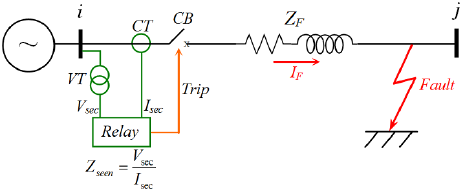
\includegraphics[width = 0.8\textwidth]{Figs/Distance.png}
            \caption{Basic schematic of distance protection~\cite{distanceFigure}}
            \label{fig:distanceFigure}
        \end{figure}
        \item Differential protection: the working principle of differential protection is that the sum of ingoing and outgoing currents in a given protected zone should be equal to zero according to Kirchhoff's law. A sum that is (significantly) different from zero indicates the presence of a fault and the necessity to trip. Due to the geographical expansions of line (dozens to hundreds of kilometres), it is necessary to have communication between both ends of a line to use differential protections. The advantage of differential protection is its high robustness and selectivity. However, it cannot act as a backup for faults outside the protected zone. It is mainly used in conjunction with distance protections for extra-high-voltage lines (400~kV in Europe) where the reliability requirements are the highest.
        \item Overcurrent protection: as the name indicates overcurrent protection disconnect the protected line when it is subject to high currents. It can either be definite-time (trips when the current is higher than a threshold for a given duration) or inverse-time (trips faster for more severe overcurrents). In transmission systems, line overcurrent protection is mostly used as (primary or backup) protection for ground faults, but distance protection is becoming more common for this application. It is also used as primary protection in some subtransmission systems and in many distribution systems~\cite{Vernova_overcurrent}.
    \end{itemize}
    \item Transformer protection: as for lines, transformers may need to be disconnected due to either internal faults or due to abnormal conditions imposed by the rest of the system. Internal faults are however rarer as transformers are less subject to external disturbances (lightning, wind). Different schemes are used to protect against internal faults and abnormal conditions:
    \begin{itemize}
        \item Internal faults: this is mainly done via differential protection thanks to its robustness and the relatively small size of transformers (a few meters vs. kilometres for lines). Other protection schemes not based on electrical variables (e.g. pressure) can also be used and are described in the reference book~\cite{HorowitzBook}.
        \item Abnormal conditions: transformers are much more sensitive too overloads than lines (overloaded lines sag, overloaded transformers lose lifespan or explode). This means that, as opposed to lines, overload protection plays an important role in transformer protection.
    \end{itemize}
    \item Generator protection: similarly to transformers, generators have to be protected against both internal faults and abnormal conditions. For electrical faults, differential protection is often used, but depending on the generator technology, many types of protection schemes can be used. Regarding abnormal conditions, the main causes of generator disconnections are listed below. It is important to note that grid codes define what are ``abnormal conditions'', i.e. define when generators should stay connected to the grid, when they are allowed to disconnect, and in some cases require them to disconnect.
    \begin{itemize}
        \item Abnormal frequency: over-frequency can cause mechanical damage in synchronous generators and their turbine; and under-frequency leads to reduce ventilation and can cause mechanical resonance. In continental Europe, generators might be quickly disconnected when frequency falls out of the 47.5-51.5~Hz range~\cite{ENTSOEgeneratorRequirements}.
        \item Low voltages: low voltage mostly affect generator auxiliary systems and indirectly affect the performance of generators. In continental Europe, generators should withstand voltage down to 0.85pu for at least 60~min~\cite{ENTSOEgeneratorRequirements}.
        \item Fault ride-through: generators should be able to stay connected when temporary faults occur in their vicinity (e.g. lightning strike on a nearby line). Ride-through requirements are defined using curves as in Figure~\ref{fig:LVRT_G99}. As long as the generator voltage stays above the curve following a disturbance, the generator must stay connected. If voltage falls below the curve (e.g. if the voltage is lower than 0.7pu more than 140ms after the occurrence of the fault), the generator is allowed to disconnect.
        \begin{figure}
            \centering
            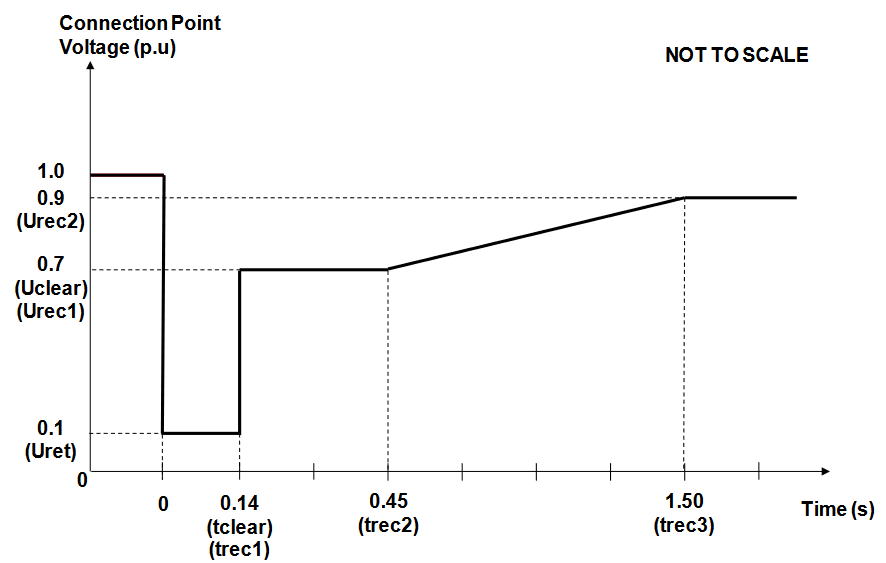
\includegraphics[width = 0.6\textwidth]{Figs/LVRT.png}
            \caption{Fault ride-through profile for large synchronous generators in the UK~\cite{G99}}
            \label{fig:LVRT_G99}
        \end{figure}
        \item Overexcitation: when a synchronous generator simultaneously produces high active and reactive power, it leads to high stator currents that can overheat the generator. When this occurs, the generator excitation will automatically be reduced after a few minutes to reduce the reactive power production and protect the generator. However, this can cause long-term voltage stability issues.
    \end{itemize}
    \item System protection: some protection systems do not aim to protect a particular element of the grid, but to protect the stability of the grid itself. Some key examples are listed below.
    \begin{itemize}
        \item Under-frequency load shedding (UFLS): UFLS relays are a last-resort solution to severe load generation imbalances following large generator disconnections or system splits. In Europe, UFLS relays disconnect load by steps when frequency falls between 49 and 48~Hz (increasingly more steps are activated the lower the frequency falls)~\cite{ENTSOE-UFLS}.
        \item Out-of-step relaying: power system swings can cause distance relays to operate. Indeed, let's consider that during a swing of the 2-generator system shown in Figure~\ref{fig:OOS}, the two generator angles are 180° from each other (the maximum value for a stable swing according to the basic equal area criterion), and that the voltage magnitude at the two generators are approximately equal. Then, these two voltages will cancel out for point that are at an equal electrical distance from the two generators. Points with zero or low voltage will be seen at faults by distance relays. These relays might then trip if they see an apparent impedance that stays in one of their zone of operation for more than the zone time delay. Out-of-step relays can distinguish faults from power swings thanks to their different timescales (faults occur in a few milliseconds, swings in hundreds of milliseconds) and can be used to block the operation of distance relays. During unstable swings, they can split the system at predefined locations with the aim of creating balanced islands. For example, the split shown in Figure~\ref{fig:OOS} would be beneficial if the active output of generator \(G_1\) is close to the sum of loads \(L_2\) and \(L_4\), and the output of \(G_3\) close to the load of \(L_5\).
        \begin{figure}
            \centering
            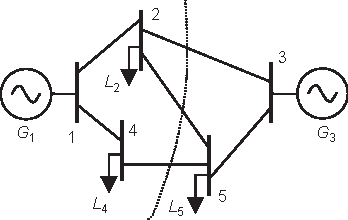
\includegraphics[width = 0.5\textwidth]{Figs/Out_of_step.pdf}
            \caption{System separation by out-of-step relays~\cite{HorowitzBook}}
            \label{fig:OOS}
        \end{figure}
        \item Other system integrity protection schemes (SIPSs)~\cite{IEEE_SIPS, CIGRE_SIPS_tutorial}: the push to operate power grids closer to their limits has led to an increasing popularity of SIPSs. SIPS are ``designed to detect abnormal system conditions and take predetermined, corrective action (other than the isolation of faulted elements) to preserve system integrity''. SIPSs can be designed to solve a wide variety of issues, and as such there are many existing SIPS designs. SIPSs can either be event-based (respond to an event, e.g. loss of a line) or response-based (respond on a system condition, e.g. loss of synchronism), and they can be either centralised (gather all needed information to a central location (e.g. the control centre) and send control signals using telecommunications) or decentralised. They are increasingly being used as part of defence plans of TSOs~\cite{CigreDefensePlan, ENTSOEdefencePlan}.
    \end{itemize}
\end{itemize}



\section{Modelling protection systems in probabilistic security assessments}
\label{sec:FMEA}

Because deterministic security assessments usually do not consider N-k contingencies nor cascading outages, they generally model protection systems in a very simplified manner. For example, for a line fault, it is generally assumed the fault will be cleared in normal time (or in backup clearing time to have a margin) by opening the line. And since no cascading outage should occur, it is assumed that no other protection system will operate.

In probabilistic assessments however, the possibility of a failure to normally clear the fault is considered. Such protection failures can lead to N-k contingencies as adjacent branches need to be disconnected to clear the fault. The impact and reasons for protection systems failing to normally clear faults is discussed in section~\ref{sec:protection_clearing}.

As cascading outages need to be simulated in probabilistic assessments, it is also important to consider the impact of protection systems beyond the clearing of the initial fault. Indeed, protection systems play a key role in the propagation of cascading outages and thus need to be modelled adequately. This is discussed in section~\ref{sec:protection_cascade}.


\subsection{Impact of protection systems after an initial fault}
\label{sec:protection_clearing}

To understand the impact and estimate the probability of protection failure to clear a fault, it is important to note that, as for any critical system, multiple layers of redundancy are used to make sure that faults are cleared in a timely manner and with minimum impact on the system. This is especially true at higher voltage levels where higher levels of redundancy are used.

Figure~\ref{fig:fault_clearing} demonstrates this with an example. In this example, there is a fault on line AB. Normally, the relays R\textsubscript{1} and R\textsubscript{5} located at both ends of the line will see this fault and respectively send tripping signals to the breakers B\textsubscript{1} and B\textsubscript{5}. This is the primary protection of line AB, and it clears the fault simply by opening both ends of the line as shown in Figure~\ref{subfig:clearing_normal}.

\begin{figure}
    \centering
    \subfloat[Clearing of the fault F by the primary protection (R\textsubscript{1} or its duplicate R\textsubscript{2}), typical clearing time: 100ms]{%
        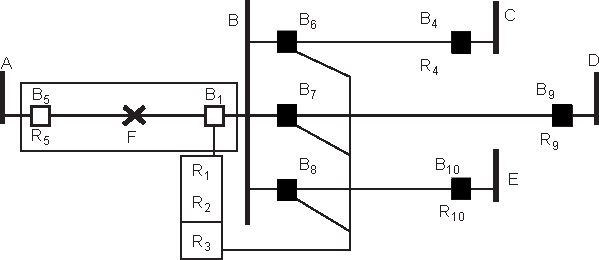
\includegraphics[width=0.7\linewidth]{Figs/Clearing_normal.pdf}
        \label{subfig:clearing_normal}
    } \\ \vskip 0.5 \baselineskip
    \subfloat[Use of local backup protection following failure to open of breaker B\textsubscript{1}, typical clearing time: 200ms]{%
        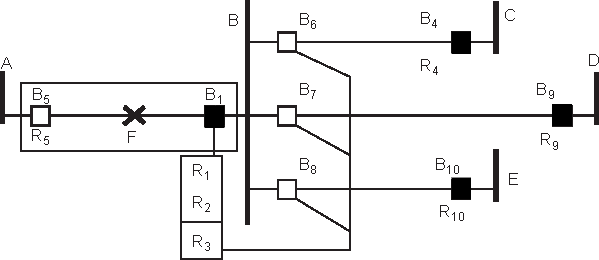
\includegraphics[width=0.7\linewidth]{Figs/Clearing_breaker.pdf}
        \label{subfig:clearing_breaker}
    } \\ \vskip 0.5 \baselineskip
    \subfloat[Fault clearing by remote backup, typical clearing time: 500ms-2s]{%
    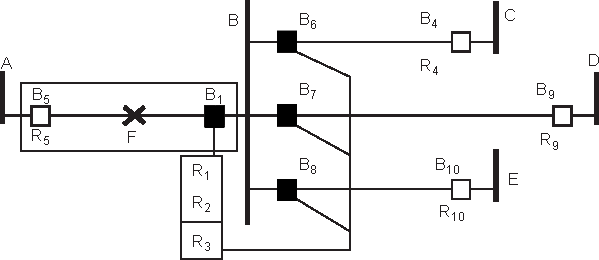
\includegraphics[width=0.7\linewidth]{Figs/Clearing_Z3.pdf}
    \label{subfig:clearing_Z3}
    }
    \caption{Duplicate primary, local backup, and remote backup protection, based on~\cite{HorowitzBook}. Black breakers are closed, white breakers are open.}
    \label{fig:fault_clearing}
\end{figure}

To increase the dependability of this scheme, elements of the primary protection can be duplicated. In this example, R\textsubscript{2} acts as a duplicate for R\textsubscript{1}. The duplicate can be identical to R\textsubscript{1} or use a different protection scheme (e.g. use of both differential and distance protection). The transducers and battery power supply can also be duplicated. The breaker is usually not duplicated due to its higher cost.

R\textsubscript{3} acts as a local backup, also called breaker failure protection. If R\textsubscript{1} or R\textsubscript{2} sends a tripping signal but B\textsubscript{1} does not open, R\textsubscript{3} will send a trip signal to B\textsubscript{6}, B\textsubscript{7} and B\textsubscript{8} as shown in Figure~\ref{subfig:clearing_breaker}. This allows for the fault clearing despite failure of breaker B\textsubscript{1} but requires the disconnection of non-faulted elements (lines BC, BD, and BE) leading to an N-4 contingency in this case. Also, breaker failure protection operates with a larger time delay than the primary protection which challenges dynamic stability.

If either

\begin{itemize}
    \item Both R\textsubscript{1} and R\textsubscript{2} fail to see the fault (and thus send no signal to B\textsubscript{1} nor to the breaker failure protection relay R\textsubscript{3})
    \item R\textsubscript{1} or R\textsubscript{2} operate, but B\textsubscript{1} fails to open and breaker failure protection (R\textsubscript{3}) fails
    \item R\textsubscript{1} or R\textsubscript{2} operate, but B\textsubscript{1} fails to open and no breaker failure protection schemes is installed
\end{itemize}
\noindent then, the remote backup protection of relays R\textsubscript{4}, R\textsubscript{9} and R\textsubscript{10} will need to be activated as shown in Figure~\ref{subfig:clearing_Z3}. This remote backup protection is often performed by zone 3 relays and thus needs even more time to clear the fault than primary or local backup protection.

The example above considered that substations each consist of a single bus single that directly connects all incident lines together, so that breaker failure protection need to open all breakers in a substation. However, different types of substation configurations can be used to reduce the impact of breaker failure (and to increase reliability in general). Figure~\ref{fig:substation} shows the most common substation configurations and how they are impacted by breaker failure.

Figure~\ref{subfig:substation_single} shows the single-bus, single-breaker substation discussed in the previous example. The substation is made of a single bus and all elements are connected to this bus through a single-breaker. This is the simplest configuration, however, if a fault occurs on one of the elements and the associated breaker fails to open, all other breakers need to open in order to isolate the fault.

At the other end of the reliability spectrum lies the two-bus, two-breaker substation configuration (Figure~\ref{subfig:substation_double}). This substation consists of two buses, and each element is connected to each bus via a breaker (so, two breakers are needed per element, hence the name). When a fault occurs on one of the elements, both its breakers need to be opened. If one breaker fails to open, all other breakers connected to the same bus will need to open to isolate the fault. However, as (non-faulted) lines are still connected to the other bus, they remain in service. In this configuration, failure of a (single) breaker does not cause the loss of additional elements. However, it requires twice as many breakers per connected elements than the previous case, so it is basically twice as expensive.

\begin{figure}
    \centering
    \subfloat[Single-bus, single-breaker substation: all lines are disconnected following breaker failure to open]{%
        \begin{minipage}{0.45\linewidth}
            \centering
            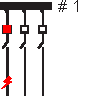
\includegraphics[height=0.15\textheight]{Figs/BFP_single_bus.pdf}
        \end{minipage}
        \label{subfig:substation_single}
    } \hfill
    \subfloat[Two-bus, two-breaker substation: bus 2 is disconnected, but all (non-faulted) lines remain connected]{%
        \begin{minipage}{0.45\linewidth}
            \centering
        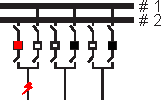
\includegraphics[height=0.15\textheight]{Figs/BFP_double_breaker.pdf}
        \end{minipage}
        \label{subfig:substation_double}
    } \\ \vskip 2 \baselineskip
    \subfloat[Two-bus, single-breaker substation: lines that are connected to the same bus as the faulted line are lost (here, it is assumed that lines 1 and 3 are initially connected to bus 1, and lines 2 and 4 to bus 2)]{%
        \begin{minipage}{0.45\linewidth}
            \centering
        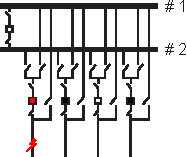
\includegraphics[height=0.2\textheight]{Figs/BFP_two_bus_one_breaker.pdf}
        \end{minipage}
        \label{subfig:substation_two_bus_one_breaker}
    } \hfill
    \subfloat[Ring substation: the bottom right line is lost due to breaker failure]{%
        \begin{minipage}{0.45\linewidth}
            \centering
        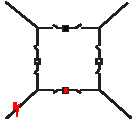
\includegraphics[height=0.2\textheight]{Figs/BFP_ring.pdf}
        \end{minipage}
    \label{subfig:substation_ring}
    } \\ \vskip 2 \baselineskip
    \subfloat[Breaker-and-a-half substation: one line is lost for failure to open of the middle breaker]{%
        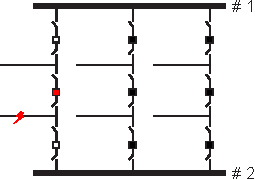
\includegraphics[width=0.45\linewidth]{Figs/BFP_half_middle.pdf}
    \label{subfig:substation_half_middle}
    } \hfill
    \subfloat[Breaker-and-a-half substation: bus 2 is disconnected, but all lines remain connected]{%
        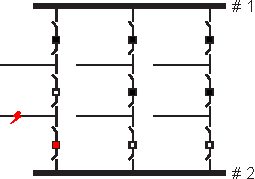
\includegraphics[width=0.45\linewidth]{Figs/BFP_half_bottom.pdf}
    \label{subfig:substation_half_bottom}
    }
    \caption{Impact of breaker failure to open in different substation configurations, based on~\cite{HorowitzBook}. All breakers are assumed initially closed in this example. Black breakers are closed, white breakers are open, and red breakers are stuck close.}
    \label{fig:substation}
\end{figure}

Figure~\ref{subfig:substation_two_bus_one_breaker} shows a two-bus, single-breaker substation. This configuration consists of two buses, but each element is normally only connected to one of the two buses (switches can change to which bus an element is connected but only when the element is not energised). A breaker connects the two buses such that all elements are connected together\footnote{The busbar coupler can be opened even without the presence of a fault in order to split the substation and change the power flows in and around the substation.}. In case of breaker failure, the breaker that connects the two buses is opened such that only elements that are connected to the same bus as the faulted element need to be disconnected. In this example (Figure~\ref{subfig:substation_two_bus_one_breaker}), breaker failure leads to N-2 contingencies, while it would have led to N-4 contingencies with the single-bus configuration.

Ring substations (Figure~\ref{subfig:substation_ring}) consist of a ring of circuit-breakers with one element connected between each pair of breakers. In this configuration, a faulted element requires two breakers to open, but breaker failure only causes the loss of one additional element.

Breaker-and-a-half substations (figures~\ref{subfig:substation_half_middle} and~\ref{subfig:substation_half_bottom}) consist of two buses linked by chains made of three breakers in series. One element is connected between the first and second, and between the second and third breaker of each chain. This configuration is called breaker-and-a-half because, on average, it requires one and a half breaker per connected element (in this example, 9 breakers for 6 elements). As shown in the figures, failure to open the middle breaker leads to the loss of one additional element, and failure to open the first or third breaker does not cause the loss of any additional element.

Modelling the possible failures of protection systems as discussed above can be done using standard reliability analysis techniques. Ref.~\cite{GridPSA, Haarla} provide many examples of event trees that describe the impact of protection failure on fault clearing. They also use fault trees to estimate the probability of the possible outcomes of a fault (normal clearing, delayed clearing, clearing with breaker failure protection, etc.) based on fault statistics of protection elements (relays, breakers, transducers, etc.) gathered in Finland and the other Nordic countries.

The discussion above has focused purely on protection system failure to clear faults, i.e. on the lack of dependability of protection systems. Another issue of protection systems is that they do not have 100\% selectivity, i.e. they will sometimes cause unnecessary trips. Unwanted trips that occur ``spontaneously'', i.e. without the occurrence of a fault, pose low risk to system security as they simply cause N-1 contingencies against which the system should normally be secure. However, unwanted trips that occur as a consequence of a fault will lead to N-2 contingencies (one element lost because it is faulted, the second because of the unwanted trip) that pose higher risks.

Modelling of unwanted trips is a complex issue. Historically, there has been much emphasis on the possibility of relays to trip due to misoperation of zone 3 distance protection caused by a timer stuck close~\cite{ZoneVulnerability, OriginalManchesterModel}. Indeed, in legacy electromechanical relays, the time-delay of zone 3 was implemented by a physical timer that could get stuck causing the zone 3 to operate without time delay. This failure mode no longer exist in numerical relays, but up until very recently, there has been little updates in the unwanted tripping models of distance relays~\cite{Alexandre_PMAPS}. Another issue caused by zone 3 was the tendency of relays to trip in high loading conditions (high loads are seen as small impedances)~\cite{3rdZoneRevisited} as seen in the US 2003 blackout. This issue has also been made less prevalent by numerical relays that can use load blinders to distinguish between remote faults and high-load conditions.

A major cause of protection misoperations is the inadvertent use of wrong settings in protection relays (this issue is actually made worse with modern relays) and design errors~\cite{ProtectionMisoperationsBian2012}. These issues are extremely difficult to model and no unwanted tripping model for modern numerical relays could be found in the literature. Unfortunately, due to lack of time, no model is proposed in this thesis either.

\begin{tcolorbox}[width=\linewidth, %sharp corners=all,
    colback=red!5!white,
    colframe=red!75!black,
    breakable,
    title=Note]
One key highlight of~\cite{GridPSA} is that, when using historical failure statistics, one should pay attention to the kind of failures that are reported. For example, ref.~\cite{GridPSA} estimates SF6 circuit breaker failure rates based on Finnish statistics (0.0028 failures to open, and 0.01 failures to reclose per year, for a total of 0.0128 failures per year) and compare it to the value published in a CIGRE report (0.012 failures per year). The two failure rate estimates are very close. However, ref.~\cite{GridPSA} distinguishes between failure to open and failure to reclose because failures to open pose a significantly greater security risk (transform N-1 contingencies into N-k ones as discussed above).

Similarly, ref.~\cite{GridPSA} reads from a report that most unwanted Finnish trips are spontaneous at the highest voltages (400 and 220~kV) and unselective at 110~kV. However, they did not have figures for unselective trips at high voltage levels which are the most critical for system security. In conclusion, careful attention should be paid to what are the failure modes considered in fault statistic reports and at what voltage levels they occurred.
\end{tcolorbox}



\subsection{Impact of protection systems during cascading outages}
\label{sec:protection_cascade}

Protection systems play a key role in the development of cascading outages. It is thus necessary to model them explicitly in the power system simulator used to study the cascading outages. All time-domain cascading simulators in the literature model the expected behaviour of the most common types of protection systems. For example, for distance relays, the associated model would compute the apparent impedance seen by the relays and would trip if this impedance stays in a protected zone for longer than its time-delay as shown in algorithm~\ref{alg:distance} (simplified for the sake of brevity). % The protection system models developed in this thesis are available online\footnote{\url{https://github.com/dynawo/dynawo/tree/master/dynawo/sources/Models/Modelica/Dynawo/Electrical/Controls/Protections}}.

\begin{algorithm}
\centering
\caption{Simplified distance protection model with a single protected zone}\label{alg:distance}
\begin{algorithmic}[1]
\State \(t_{Breaker} \gets\) 80ms
\State \(t_{ZoneDelay} \gets\) 300ms (typical value for zone 2, other values should be used for different zones)
\State \(\underline{Z} \gets \dfrac{\underline{U}}{\underline{I}}\)

\\
\If{\(\underline{Z}\) is in the protected zone and \(t_{Arming} = \infty\)}
    \State \(t_{Arming} \gets t\)
\ElsIf{\(\underline{Z}\) is outside the protected zone}
    \State \(t_{Arming} \gets \infty\)
\EndIf

\\
\If{\(t > t_{Arming} + t_{ZoneDelay}\)}
    \State \(t_{Trip} \gets t\)
\EndIf

\\
\If{\(t > t_{Trip} + t_{Breaker}\)}
    \State Disconnect protected element
\EndIf

\end{algorithmic}
\end{algorithm}

Multiple types of protection systems can operate during cascading outages and should thus be adequately modelled. Based on historical disturbances, ENTSO-E listed the types of protections most likely to operate during cascading outages~\cite{ENTSOEdefencePlan}:

\begin{itemize}
    \item Distance protection (first and higher zones)
    \item Overcurrent relays
    \item Differential relays
    \item Under-frequency load shedding
    \item Under-voltage load shedding
    \item Generator protection
    \begin{itemize}
        \item Under- and over-voltage relays
        \item Under- and over-frequency relays
        \item Loss-of-field relays
        \item Volt/Hz over-excitation relays
        \item Generator backup relays
    \end{itemize}
\end{itemize}

Moreover, as discussed above, there are three additional complexities that can be considered in the modelling of protection systems:

\begin{itemize}
    \item Missing trips: protection systems might not trip when expected to either due to a failure of an element of the protection system (relay, breaker), or due to a misoperation of the relay.
    \item Unwanted trips: relays might send tripping signals when not expected to.
    \item Sensitivity of cascading outages to small changes in protection behaviour: small changes in the timing of protection systems operation can impact the order in which protection systems operate, and potentially vastly impact the cascade evolution.
\end{itemize}

Missing trips caused by relay or breaker failures can relatively easily be modelled as has been done in the DCAT tool~\cite{DCATphase1} and in approaches based on dynamic event trees~\cite{TwoLevelPSA}. In DCAT, when a protection system operates during a cascade, two possible branches of the simulation are created: one where the protection actually operates and one where it fails to. The frequency associated with each branch is weighted according to the probability of the protection system to operate (for the former branch) or to fail (for the latter)\footnote{As protection systems are often designed to protected individual elements and not the grid itself, it can be argued that, once a cascade is initiated, protection failures might not necessarily negatively impact system stability. And, since protection failures are unlikely, their contribution to the risk might be negligible. Indeed, chapter~\ref{ch:DPSA} demonstrates that for the considered test system, protection failures to operate during cascading outages do not significantly impact the risk estimate. However, this might be system dependent and the argument is of course not valid for SIPSs.}. This probability can be estimated based on standard reliability techniques (e.g. fault trees).

During cascading outages, power system operate in very degraded states which can cause protection system misoperations leading to both missing and unwanted trips. The most common misoperations have been reported by the IEEE Power System Relaying and Control Committee (PSRC)~\cite{ProtectionFailuresDemetrios, PSRCreportProtectionMisop, PSRCreportSummaryProtectionMisop} and are listed below.

The main contributor of relay misoperations is again (zone 3) distance protection. Indeed, distance protection can trip following power swings, high loads, and low-voltage conditions\footnote{In the case of low voltages, loads will tend to increase the current they draw, trying to partially maintain a constant power draw, and thus leading to low-voltage, high-current conditions. Such conditions are seen as small apparent impedances by distance relays that are thus likely to trip}. However, such misoperations can easily be modelled by explicitly representing the relays in a time-domain simulator (as shown in the simplified algorithm~\ref{alg:distance}). Of course, if some distance relays have load blinders and power swing blocking functionality, these should be modelled too. Similarly, although less often used on the high-voltage levels, overcurrent protections can also trigger during power swings, high-load, or low-voltage conditions.

Another issue is the operation of backup ground overcurrent relays of highly-loaded untransposed lines. Indeed, untransposed lines can have current imbalances up to 10\% creating a zero sequence component. This can be enough to trigger ground overcurrent relays in case of high loads (or transient high currents). In modern relays however, this issue can be alleviated by restraining the ground overcurrent relays by a fraction of the positive sequence current.

Frequency deviations can cause inaccuracies in the evaluation of phasors. However, as frequency should always stay within 5\% of its nominal value (otherwise the system is already on its way to a complete blackout), the associated errors are small. These errors also depends on which frequency tracking scheme is used by the relays and are thus simply modelled as measurement errors in this thesis. They are thus handled in section~\ref{sec:protection_uncertainty}.

Finally, ref.~\cite{ProtectionFailuresDemetrios, PSRCreportProtectionMisop, PSRCreportSummaryProtectionMisop} discusses issues related to the polarisation of relays (voltage angle estimated from past measurement when voltages too low for an accurate measurement). However, as these issues mainly affect legacy mho relays, they are not considered in this thesis.



\section{Handling uncertain protection behaviour in simulations of cascading outages}
\label{sec:protection_uncertainty}

\begin{tcolorbox}[width=\linewidth, sharp corners=all,
    colback=white!80!black,
    colframe=white!80!black]
This section is partly based on the following publication:
\begin{itemize}
    \item \fullcite{ISGT2023_Protections}
\end{itemize}
\end{tcolorbox}

During fast cascading outages, many protection systems can operate in a very short period of time. This renders the simulation of cascading outages quite complex as small modelling uncertainties can potentially have high impacts on which protection systems actually operate and in which order, therefore strongly affecting how the cascade propagates.

One example of such fast cascade occurred on 8 January 2021 and led to the separation of the Continental Europe power system into two synchronous regions as shown in Figure~\ref{fig:split2021}. The split occurred when there were high power flows from South-Eastern Europe to North-Western Europe and was initiated by the decoupling of two busbars in the Ernestinovo substation due to busbar coupler overload protection. (This event can be loosely classified as an N-2 event as it interrupted SE-NW flows along two axis (Ugljevik-Zerjavinec and Sremska Mitrovica-Pecs) as shown in Figure~\ref{fig:split2021_timeline}.) High power flows and the reduced transmission capacity caused by the busbar coupler trip led to angle instability and a subsequent split of the system in a cascading manner.

\begin{figure}
    \centering
    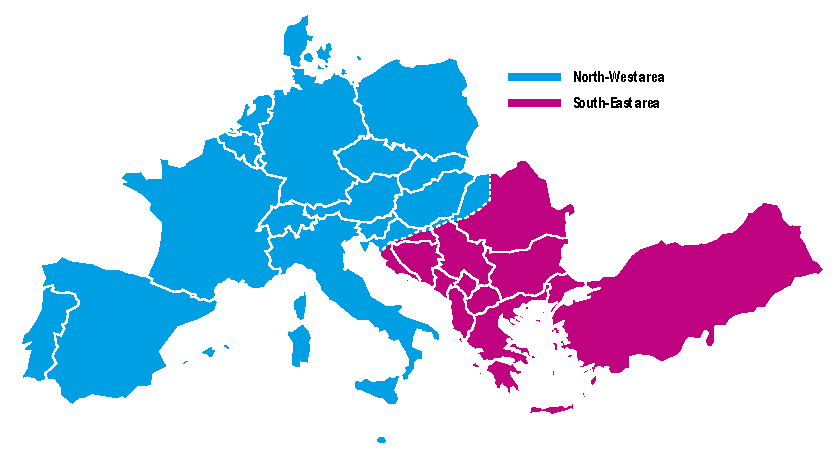
\includegraphics[width = 0.7\textwidth]{Figs/SystemSplit2021.pdf}
    \caption{Resulting two synchronous areas after the 8 January 2021 European system split~\cite{ENTSOESplitJan2021}}
    \label{fig:split2021}
\end{figure}

\begin{figure}
    \centering
    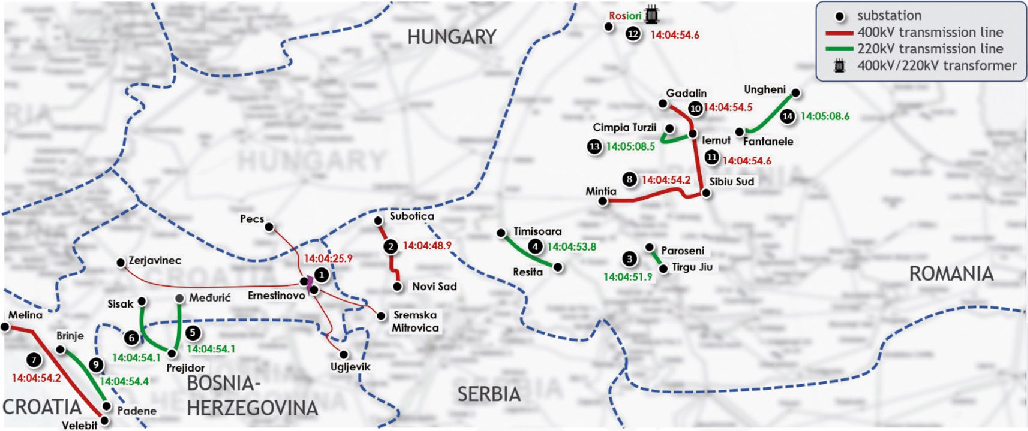
\includegraphics[width = \textwidth]{Figs/SystemSplitTimeline2021.pdf}
    \caption{Geographical location of elements tripped during the 8 January 2021 European system split~\cite{ENTSOESplitJan2021}. Trip of 110~kV lines are not represented.}
    \label{fig:split2021_timeline}
\end{figure}

\begin{table}
\centering
\caption{Timeline of events that led to the 8 January 2021 European system split~\cite{ENTSOESplitJan2021}. Approximately 15 110~kV lines were tripped but are not listed.}
\label{tab:split_timeline}
\begin{adjustbox}{max width=\textwidth}
\begin{tabular}{@{}lllllll@{}}
\toprule
No & Country & delta [s] & Substation 1 & Substation 2   & Voltage [kV] & Reason                                                 \\ \midrule
1a & Croatia & 0         & Ernestinovo  &                & 400          & Busbar coupler overload protection                     \\
1b & Croatia & 2.6       & Ernestinovo  &                & 400/110      & Overload protection of both 400 / 110 kV transformers  \\
2  & Serbia  & 23        & Subotica     & Novi Sad       & 400          & Overload protection 20s 2nd zone                       \\
3  & Romania & 26        & Paroșeni     & Târgu Jiu Nord & 220          & Distance protecton starting zone 2.4 s                 \\
4a & Romania & 27.9      & Reşiţa       & Timişoara      & 220          & Distance protection 0.4 s                              \\
4b & Romania & 27.9      & Reşiţa       & Timişoara      & 220          & Distance protection 0.4 s breaker L1 failure           \\
5  & Bosnia  & 28.2      & Prijedor     & Međuriċ        & 220          & Distance protection out-of-step protection             \\
6  & Bosnia  & 28.2      & Prijedor     & Sisak          & 220          & Distance protection out-of-step protection             \\
7  & Croatia & 28.3      & Melina       & Velebit        & 400          & Distance protection zone 3                             \\
8  & Romania & 28.3      & Mintia       & Sibiu          & 400          & Distance protection power swing condition              \\
9  & Croatia & 28.5      & Brinje       & Padene         & 220          & Distance protection zone 1                             \\
10 & Romania & 28.6      & Gădălin      & Iernut         & 400          & Distance protection power swing condition zone 2 0.4 s \\
11 & Romania & 28.7      & Sibiu Sud    & Iernut         & 400          & Distance protection zone 3 reverse 0.6 s               \\
12 & Romania & 28.7      & Roşiori      &                & 400/220      & Distance protection power swing condition              \\
13 & Romania & 42.6 & Iernut & Câmpia Turzii & 220 & Distance protection zone 2 power swing conditions \\
14 & Romania & 42.7      & Fântânele    & Ungheni        & 220          & Distance protection zone 2 power swing conditions      \\ \bottomrule
\end{tabular}
\end{adjustbox}
\end{table}

The trips that led to the system separation are listed in Table~\ref{tab:split_timeline} and shown in Figure~\ref{fig:split2021_timeline}. As can be seen from the table, events 4 to 12 occur in less than a second showing the possibility of different tripping orders. Also, it demonstrates the importance of distance protection in the development of cascading outages. Finally, it can be noted that some TSOs use power swing blocking for distance protection and some do not.

Similarly, although not the focus of this thesis, slow cascades are also affected by modelling uncertainties. The tripping of overloaded lines is caused by lines sagging into vegetation and thus depends on uncertain parameters as vegetation height, temperature and wind. % The order of trips can thus also be affected by uncertainties.

A common approach to handle uncertainties is to use Monte Carlo (MC) simulations and their derivatives. Notably, in~\cite{TwoLevelPSA}, fast cascading outages are simulated with dynamic event trees where each possible realisation of a protection system behaviour leads to different possible branches. In~\cite{SequencesRelaySobol}, the order of protection system operation is encoded in a matrix that is then used with extended forms of variance-based sensitivity estimators to rank how sensitive cascading outages are to different power system variables.

The issue with MC techniques is that they can be computationally expensive. This poses an important challenge for this thesis as systematic probabilistic dynamic security assessments require to simulate many cascading outage scenarios. To alleviate this challenge, a simple indicator has been developed to predict which cascading outage scenarios are sensitive to protection-related uncertainties and which are not. MC simulations then only have to be performed for the former limiting their impact of computation time. The simple indicator is presented in section~\ref{sec:protection_indicator}. It is applied on a standard test system with a set of protection systems described in section~\ref{sec:protection_test_case}, and its performance is discussed in section~\ref{sec:protection_results}.


\subsection{Identifying sensitive scenarios}
\label{sec:protection_indicator}

The objective of the indicator is to predict which scenarios (combination of a given initial system state and of a contingency) lead to cascading outages whose evolution is sensitive to protection-related uncertainties and which scenarios do not.

The indicator is constructed by building and comparing two extreme trip sequences. The first sequence is generated by simulating the system with protection systems operating as slowly as possible (leading to a so-called ``slow sequence'' of tripping events (Fig.~\ref{subfig:slowSeq})). This is done by selecting, in the distribution of the protection parameters, the values that lead to the slowest protection operations. For example, for a distance protection, this would imply taking the smallest value of the size of the zones of operation, and the largest value for the opening time of the circuit breaker. The second sequence is generated by simulating the system with fast protection systems (leading to a ``fast sequence'' of tripping events).%\footnote{Actually, it is sufficient to only accelerate the operation of distance protections when generating the faster sequence. According to our tests, accelerating only the distance protections or all protections leads to the same performance of the indicator. This can be explained by the fact that, most often, distance protections are the ones that initiate fast cascading outages~\cite{ENTSOESplitJan2021, ENTSOEIbericSplit2021}.}

\begin{figure}
    \centering
    \subfloat[Slow sequence (reference)]{%
        \begin{tikzpicture}[scale=1.5]
        % draw horizontal line
        \draw (0,0) -- (7,0);

        % draw vertical lines
        \foreach \x in {0,1,4.5,6,7}
          \draw (\x cm,3pt) -- (\x cm,-3pt);

        % draw nodes
        \draw (1,0) node[below=3pt] {$ 1_a $};
        \draw (4.5,0) node[below=3pt] {$ 2_a $};
        \draw (6,0) node[below=3pt] {$ 3_a $};
        \end{tikzpicture}
        \label{subfig:slowSeq}
        } \\ \vskip\baselineskip
    \subfloat[Fast sequence for which the system is unlikely to be affected by protection-related uncertainties]{%
        \begin{tikzpicture}[scale=1.5]
        % draw horizontal line
        \draw (0,0) -- (7,0);

        % draw vertical lines
        \foreach \x in {0,1,4,5.5,7}
          \draw (\x cm,3pt) -- (\x cm,-3pt);

        % draw nodes
        \draw (1,0) node[below=3pt] {$ 1_b $};
        \draw (4,0) node[below=3pt] {$ 2_b $};
        \draw (5.5,0) node[below=3pt] {$ 3_b $};
        \end{tikzpicture}
        \label{subfig:negative}
     } \\ \vskip\baselineskip
    \subfloat[Fast sequence likely to be affected: \(3_c\) occurs before \(2_a\)]{%
        \begin{tikzpicture}[scale=1.5]
        % draw horizontal line
        \draw (0,0) -- (7,0);

        % draw vertical lines
        \foreach \x in {0,1,2,3,7}
          \draw (\x cm,3pt) -- (\x cm,-3pt);

        % draw nodes
        \draw (1,0) node[below=3pt] {$ 1_c $};
        \draw (2,0) node[below=3pt] {$ 2_c $};
        \draw (3,0) node[below=3pt] {$ 3_c $};
        \end{tikzpicture}
        \label{subfig:order}
    } \\ \vskip\baselineskip
    \subfloat[Fast sequence likely to be affected: a new event (\(4_d\)) occurs]{%
        \begin{tikzpicture}[scale=1.5]
        % draw horizontal line
        \draw (0,0) -- (7,0);

        % draw vertical lines
        \foreach \x in {0,1,4.5,6,6.5,7}
          \draw (\x cm,3pt) -- (\x cm,-3pt);

        % draw nodes
        \draw (1,0) node[below=3pt] {$ 1_d $};
        \draw (4.5,0) node[below=3pt] {$ 2_d $};
        \draw (6,0) node[below=3pt] {$ 3_d $};
        \draw (6.5,0) node[below=3pt] {$ 4_d $};
        \end{tikzpicture}
        \label{subfig:new_event}
    }
    \label{fig:fig}
    \caption{Classification of tripping sequences according to the proposed indicator}
\end{figure}

The indicator predicts that a scenario is sensitive to uncertainties if either

\begin{itemize}
    \item Comparing the two sequences shows the possibility for two events to be swapped (Figure~\ref{subfig:order}).
    \item If one event occurs in one sequence but not in the other (Figure~\ref{subfig:new_event}).
\end{itemize}

The first condition detects cases where uncertainties can affect the order of protection system operations. And the second detects ``near-misses'', i.e. cases where one protection does not operate but is very close to (e.g. for a distance protection, the apparent impedance enters the protected zone but leaves just before the protection time delay). Regarding the first condition, it should be noted that events could occur in the same order in both the slow and fast sequences (as shown in Figures~\ref{subfig:slowSeq} and~\ref{subfig:order}) but still indicate the possibility for uncertainties to affect the order of protection system operations. Indeed, in Figure~\ref{subfig:order}, the event \(3_c\) occurs before \(2_a\) highlighting the possibility for events \(2\) and \(3\) to be swapped.

To avoid having to perform two simulations for each scenario (one with slower and one with faster protection systems), it is also possible to perform a single simulation with models of both slower and faster protections. In this case, the faster protection systems should not be connected to a circuit breaker, so that they do not affect the system evolution but still generate the log messages needed to generate the fast sequence. This is an approximation (the fast sequence is based on the system evolution with slow protection), but it has a small impact on the precision of the indicator (as shown in section~\ref{sec:protection_results}) and requires only one simulation instead of two.


\subsection{Test case and protection system models}
\label{sec:protection_test_case}

The test case used in this example is the IEEE 39-bus test system~\cite{IEEE39} shown in Figure~\ref{fig:IEEE39} with dynamic data taken from~\cite{IEEE39Dynamic} and a few minor modifications made to make the system more realistic~\cite{ISGT2023_Protections}.

\begin{figure}
    \centering
    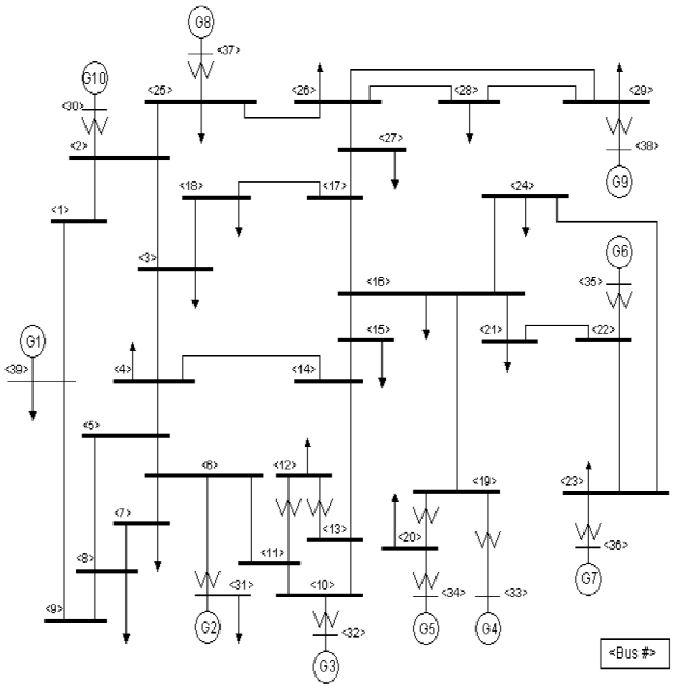
\includegraphics[width=0.7\textwidth]{Figs/IEEE39.png}
    \caption{IEEE 39 bus system~\cite{IEEE39figure}}
    \label{fig:IEEE39}
\end{figure}

The load model has been changed to a restorative exponential load model, i.e.

\begin{equation}
\label{eq:restorative_load_model_1}
P = P_0 \left(\frac{U}{U_f}\right)^2, \quad Q = Q_0 \left(\frac{U}{U_f}\right)^2
\end{equation}
\noindent where \(P\) (resp. \(P_0\)) and \(Q\) (\(Q_0\)) are the (initial) active and reactive power consumption of the load, \(U\) is the voltage at the load bus, and \(U_f\) satisfies

\begin{equation}
\label{eq:restorative_load_model_2}
t_f \frac{dU_f}{dt} = U - U_f, \quad U_f \ge 0.5
\end{equation}
\noindent where \(t_f\) is the restoration time of the load. Three values of this parameter are used in this example: 1s, 5s, and infinite (i.e. non-restorative load) in order to study different kinds of cascading outages.

As the standard IEEE 39-bus system has no protection models, the following protection systems were added:

\begin{itemize}
    \item Line protection: distance protection is used on all lines and can trip during out-of-step conditions (no power swing blocking functionality is implemented\footnote{As seen in Table~\ref{tab:split_timeline}, some TSOs use power swing blocking and some do not. Power swing blocking and tripping would probably make the cascade propagation process a bit less sensitive to uncertainties as it would force system splits to happen along predefined corridors.}). Simple triangular zones are used as shown in Figure~\ref{fig:zones}. The reach of these zones are defined as
    \begin{IEEEeqnarray}{rCl}
        X_2 & = & \max(0.9 (X + 0.85 X_{short\_adj}), 1.15 X) \\
        R_2 & = & X_2 \\
        X_3 & = & X + 1.15 X_{long\_adj} \\
        R_3 & = & X_3
    \end{IEEEeqnarray}
    \noindent where \(X_i\) and \(R_i\) are respectively the inductive and resistive reaches of zone \(i\), \(X\) is the impedance of the protected line, \(X_{short\_adj}\) is the impedance of the shortest adjacent line, and \(X_{long\_adj}\) is the impedance of the longest adjacent line. The time delays for zone 2 and 3 are respectively 300 and 600ms. Once a tripping signal is sent, it is assumed that the circuit breaker needs 80ms to open. Zone 1 is not explicitly modelled. In a practical application, it would be best to use more realistic quadrilateral zones and to represent zone 1. Load blinders are not considered in this example as the IEEE 39-bus network is not subject to high power flows (i.e. in normal operation, the apparent impedance seen by relays is far from the protected zone). They will be modelled in the test case in chapter~\ref{ch:DPSA}.
    \item Generator protection: generators are automatically disconnected whenever the voltage at the generator bus drops below 0.85~pu for more than 1.5s~\cite{ENTSOEgeneratorRequirements}, when their frequency goes outside the [47.5, 52.5]~Hz range, or when their internal angle is larger than 225°.
    \item System protection: a 10-step Under-Frequency Load Shedding (UFLS) scheme is used to maintain the frequency balance as for ENTSO-E recommendations~\cite{ENTSOE-UFLS}. The first step disconnects 10\% of the load when the frequency drops below 0.98~pu. The following steps disconnect 5\% of the load each time the frequency drops by an additional 0.02~pu. All steps are thus activated for frequencies below 0.962~pu and the associated load shedding is 55\%.
\end{itemize}

\begin{figure}
    \centering
    \begin{tikzpicture}% [scale=2]
    \begin{axis}[
        % unit vector ratio*=4 1 1,
        % ticklabel style = {font=\tiny},
        % xticklabel style = {yshift=4ex},
        axis x line=center,
        axis y line=middle,
        xtick={1.2,2.5},
        xticklabels={\(R_2\),\(R_3\)},
        xticklabel style = {xshift=0.25cm},
        ytick={1.2,2.5},
        yticklabels={\(X_2\),\(X_3\)},
        yticklabel style = {yshift=0.25cm},
        xmin = -3,
        xmax = 3,
        ymin = -3,
        ymax = 3,
    ]
    \coordinate (A2) at (1.2, -1.2);
    \coordinate (B2) at (1.2, 1.2);
    \coordinate (C2) at (-1.2, 1.2);

    \coordinate (A3) at (2.5, -2.5);
    \coordinate (B3) at (2.5, 2.5);
    \coordinate (C3) at (-2.5, 2.5);

    \draw[-] (A2) -- (B2);
    \draw[-] (B2) -- (C2);
    \draw[-] (C2) -- (A2);

    \draw[-] (A3) -- (B3);
    \draw[-] (B3) -- (C3);
    \draw[-] (C3) -- (A3);

    \end{axis}
    \end{tikzpicture}
    \caption{Definition of simplified triangular zones for distance relays}
    \label{fig:zones}
\end{figure}

As this thesis focuses on short-term stability, protection systems that operate with a delay larger than a minute (overload protection, over-excitation limiters, etc.) are not modelled. Also, differential protection is not explicitly modelled in the simulator as it should only operate to clear the initial fault (whose clearing is typically ``hard-coded'' in the simulation) and not during the cascade.

The sources of uncertainty considered are listed below. Due to lack of data, uniform distributions are used to model all sources, although any distribution could be used.

\begin{itemize}
    \item The measurement of apparent impedances has an accuracy of 10\%.
    \item Generators are allowed to disconnect for voltages below 0.85~pu (lasting more than 1.5s) but are not requested to do so~\cite{ENTSOEgeneratorRequirements}. We thus consider that they will disconnect for voltages in the [0.8, 0.85~pu] range.
	\item The internal angle of generators is measured with an accuracy of 10°.
	\item Generators can disconnect up to 0.5~Hz before or after the threshold of under-/over-speed protection.
	\item The opening time of circuit breakers (for all protection systems mentioned above) can vary by up to 10ms (half a cycle) around the average value.
\end{itemize}

In order to trigger cascading outages, it is necessary to consider severe initiating events. In this example, the initiating events considered are line three-phase faults followed by a circuit breaker failure. For the sake of simplicity, it is assumed that the breaker failure relay can isolate the fault by disconnecting a single adjacent line (possible with breaker-and-a-half substations which is the most common extra-high voltage configuration~\cite{HorowitzBook}). Faults are cleared in 100ms on the side with healthy breakers and in 200ms on the opposite side. In total, 228 possible N-2 contingencies are considered\footnote{There are 34 lines, we consider that faults occur near one of the two line ends, and that breaker failure can occur on either end of the line. Also, since there are no standard substation configurations for the IEEE 39-bus system, we consider that breaker failure protection can disconnect any of the lines adjacent to the faulted breaker.}. Since the focus is on fast cascades, simulations are run for 60s\footnote{The simulation could be run for longer if an electrical steady-state is not reached after 60s as done in~\cite{DCATphase1, MCDETasTool}}.


\subsection{Results}
\label{sec:protection_results}

\subsubsection{Indicator accuracy}

To evaluate the accuracy of the indicator, all contingencies have been simulated with 50 MC samples of the protection parameters, considering a contingency to be sensitive to protection-related uncertainties if different samples led to different consequences in terms of load shedding (i.e. non-zero standard deviation). The prediction of the indicator has then been compared to these MC simulations. Table~\ref{tab:indicator} shows that the indicator has very low false negative and false positive rates, i.e. there are only few contingencies that are sensitive to protection-related uncertainties but not identified by the indicator (false negatives), and few contingencies that are not sensitive but highlighted by the indicator (false positives).

The table also shows the false negative rate computed by looking only at the contingencies whose consequences have a non-negligible standard deviation (here defined as higher than 5\% of the total load). And actually, this rate is 0, so the indicator misses none of the contingencies with non-negligible standard deviation. It can thus be expected that if this indicator is applied in the context of a probabilistic security assessment (as will be done in chapter~\ref{ch:DPSA}), the indicator will be able to identify the scenarios for which MC simulations need to be performed to have an accurate risk estimate, while avoiding unnecessary simulations on the other scenarios.

% 72, 39, 22 positives (not necessarily true positives) out of 228

% 5\% just happens to be an UFLS step

\begin{table}
\centering
\caption{Performance of the proposed indicator}
\label{tab:indicator}
\vspace{-0.3cm}
\begin{tabular}{@{}llll@{}}
\toprule
Load model      & FN (\(\ge\) 5\%) & FN     & FP            \\ \midrule
1s              & 0\% (0/37)  & 6\% (3/52)  & 13\% (23/176) \\
5s              & 0\% (0/19)  & 4\% (1/27)  & 6\% (13/201)  \\
Non-restorative & 0\% (0/10)  & 0\% (0/15)  & 3\% (7/213)   \\ \bottomrule
\multicolumn{4}{l}{\footnotesize FN (\(\ge\)5\%): False Negative with standard deviation of load shedding} \\
\multicolumn{4}{l}{\footnotesize higher than 5\%, FN: False Negative, FP: False Positive}                \\
\end{tabular}
% \end{table}
\bigskip
% \begin{table}
\centering
\caption{Performance of a consequence-only indicator}
\label{tab:indicator-consequence-based}
% \vspace{-0.2cm}
\begin{tabular}{@{}llll@{}}
\toprule
Load model & FN (\(\ge\)5\%)  & FN & FP        \\ \midrule
1s              & 41\% (15/37) & 40\% (21/52) & 1\% (1/176) \\
5s              & 37\% (7/19)  & 44\% (12/27) & 0\% (1/201) \\
Non-restorative & 10\% (1/10)  & 20\% (3/15)  & 0\% (1/213) \\ \bottomrule
\end{tabular}
\end{table}

The use of very different load models allows covering different types of cascading phenomena. Indeed, the case study with the non-restorative load model leads to very short cascading outages (at most one or two trips occur in most simulations). In this case, most of the sensitivity is caused by ``near-misses'' (when a protection system is close to operate but it just below its threshold). Sensitive contingencies are thus mostly detected via the presence of additional event(s) in the faster sequence (as defined in Fig.~\ref{subfig:new_event}). Actually, the indicator identifies 22 sensitive contingencies (out of 48 that have non-zero average consequences), and in all 22, there are additional event(s) in the fast sequence. In only 9 of them, the order of operations can be impacted by uncertainty.

On the other hand, the case study with the 1s-restorative load model can be subject to longer cascades (with up to dozens of tripping events) that often lead to complete blackouts. In this case, sensitivity is caused by both ``near-misses'' and potential changes in the order of protection operations (the latter being detected as explained in Figure~\ref{subfig:order}). 72 sensitive contingencies are identified (out of 147 that have non-zero average consequences): 64 with near-misses and 18 with variable protection order.

Figure~\ref{fig:IEEE39_sequences} illustrates this for the N-2 contingency of lines 5-6 and 6-7 (for the 1s-restorative load case, and initial fault near bus 5). When this contingency is simulated with slow protection systems (slow sequence, Figure~\ref{subfig:slow_sequence}), four distance protections operate (events 3 to 6), leading to the system splitting in three islands as shown in Figure~\ref{subfig:split_slow}. One of the islands has two loads (at buses 7 and 8) but no generators and is thus lost. The other two islands remain stable.

From the same simulation, a fast sequence can be estimated if models of fast protections are included (but not connected to breakers to not affect the system evolution). This estimated sequence is shown in Figure~\ref{subfig:estimated_fast_sequence}. This sequence has two additional distance trips (events 7 and 8) compared to the slow sequence indicating a sensitivity of the contingency to protection-related uncertainties. The occurrence of event 7 in the fast sequence is explained by Figure~\ref{fig:IEEE_split_RX_plot}. This is because in the fast sequence, the distance protection of line 13-14 is assumed to have a slightly larger reach. The apparent impedance seen by the relay thus stays a bit longer in the protected zone which causes the protection to trip.

\begin{figure}
\centering
\begin{tikzpicture}
\pgfplotsset{width=0.8\linewidth}
\begin{axis}[
    group style={
        group name=my plots,
        group size=2 by 1,
        ylabels at=edge left,
        yticklabels at=edge left,
        vertical sep=20pt,
    },
    xlabel={\(R\) [pu]},
    ylabel={\(X\) [pu]},
    xmin=-0.1, xmax=0.39,
    ymin=-0.061, ymax=0.061,
    xticklabel style={/pgf/number format/fixed},
    yticklabel style={/pgf/number format/fixed},
    scaled x ticks=false,
    scaled y ticks=false,
    tickpos=left,
    ytick align=outside,
    xtick align=outside,
    table/col sep=comma,
]
% \nextgroupplot
\addplot+ [mark=none, dashed, dash pattern=on 6pt off 6pt] table [x=R,y=X] {Figs/IEEE_split_slow.csv};

\coordinate (A1) at (0.03154945935727788, -0.03154945935727788);
\coordinate (B1) at (0.03154945935727788, 0.03154945935727788);
\coordinate (C1) at (-0.03154945935727788, 0.03154945935727788);
% \node [anchor=east] (slow) at (C1) {Slow protection};

\draw[-] (A1) -- (B1);
\draw[-] (B1) -- (C1);
\draw[-] (C1) -- (A1);


%\nextgroupplot
% Superposition of dashed lines from https://tex.stackexchange.com/a/131817
\addplot+ [mark=none, dashed,dash pattern=on 6pt off 6pt,dash phase=6pt] table [x=R,y=X] {Figs/IEEE_split_fast.csv};

\coordinate (A3) at (0.03856045032556186, -0.03856045032556186);
\coordinate (B3) at (0.03856045032556186, 0.03856045032556186);
\coordinate (C3) at (-0.03856045032556186, 0.03856045032556186);

\draw[-] (A3) -- (B3);
\draw[-] (B3) -- (C3);
\draw[-] (C3) -- (A3);
\node at (axis cs:0.0424109277580345,0.0312666883066816) [anchor=west, align=left] {Trip};
\node at (axis cs:0.0424109277580345,0.0312666883066816) [circle, fill, inner sep=1.5pt] {};

\node at (axis cs:0.0382912822075786,0.0219691705198084) [anchor=west, align=left] {Trip\\signal};
\node at (axis cs:0.0382912822075786,0.0219691705198084) [circle, fill, inner sep=1.5pt] {};

\node at (axis cs:0.356189296220075,-0.00668263904273035) [anchor=south, align=left] {Initial\\point};
\node at (axis cs:0.356189296220075,-0.00668263904273035) [circle, fill, inner sep=1.5pt] {};

\node at (axis cs:0.0160208226576352,-0.0518139264706419) [anchor=east, align=left] {Fault\\incidence};
\node at (axis cs:0.0160208226576352,-0.0518139264706419) [circle, fill, inner sep=1.5pt] {};

\node at (axis cs:0.0557547773071578,-0.000774513562478557) [anchor=north west, align=left] {Fault clearing};
\node at (axis cs:0.0557547773071578,-0.000774513562478557) [circle, fill, inner sep=1.5pt] {};

% \node at (axis cs:0.0110064179359231,-0.0310501831892437) [anchor=east, align=left] {Partial\\clearing};
% \node at (axis cs:0.0110064179359231,-0.0310501831892437) [circle, fill, inner sep=1.5pt] {};

\addlegendentry{Slow sequence}
\addlegendentry{Fast sequence}

\end{axis}
\end{tikzpicture}
\caption{Apparent impedance seen by the distance protection relay on side 2 of line 13-14 (protection causing event 7) following the N-2 contingency of lines 5-6 and 6-7 (1-s restorative load case). Triangular shapes represent the zone 3 of the protection with either ``slow'' settings (smaller zone) or ``fast'' settings (larger zone). The protection only trips in the fast sequence.}
\label{fig:IEEE_split_RX_plot}
\end{figure}

Figure~\ref{subfig:fast_sequence} shows the fast sequence that would actually be obtained by rerunning the simulation with fast protection systems. In this case, the additional distance protection operation of event 7 leads to a different system evolution with the system splitting in four islands instead of three (as shown in Figure~\ref{subfig:split_fast}). This causes high imbalances and the collapse of three of the four islands. Only the island with generator 1 (bus 39) survives because it represents an interconnection and thus has very high inertia. The fast sequence thus leads to an almost complete blackout while the slow one only leads to the loss of two loads.

Because of the different system evolution, some events that occurred in the slow sequence (event 4) and in the estimated fast sequence (events 4 and 8) do not happen in the fast sequence. The fast sequence estimated from the simulation of the slow one (Figure~\ref{subfig:estimated_fast_sequence}) is thus inaccurate. However, it allows identifying that the contingency is sensitive to protection-related uncertainties which is the objective of the indicator. In any case, MC simulations are needed to accurately estimate the risk associated with sensitive contingencies, but they can be avoided when the indicator predicts they are not sensitive.

\afterpage{%
\clearpage% Flush earlier floats (otherwise order might not be correct)
\begin{figure}
\centering
\subfloat[Slow sequence]{%
\begin{tikzpicture}[xscale=9]
\def\lt{0.3} % tick length
% help functions
\def\yearArrowLabel(##1,##2,##3,##4){
    \def\xy{{##1}}
    \pgfmathparse{int(##2*100)}
    \ifnum \pgfmathresult<0
    \def\yyp{{(\lt*(0.90+##2))}}
    \def\yyw{{(\yyp-\lt*##3)}}
    \draw[<-,thick,black,align=center] (\xy,\yyp) -- (\xy,\yyw) node[below,black] at (\xy,\yyw) {##4};
    \else
    \def\yyp{{\lt*(0.10+##2)}}
    \def\yyw{{(\yyp+\lt*##3)}}
    \draw[<-,thick,black,align=center] (\xy,\yyp) -- (\xy,\yyw) node[above,black] at (\xy,\yyw) {##4};
    \fi}
% axis
\draw[->,thick] (-0.03,0) -- (1.53,0);
% ticks
\foreach \tick in {0,0.5,...,1.5}{
    \def\x{{\tick}}
    \draw[thick] (\x,0.5*\lt) -- (\x,-0.5*\lt) node[below] {\x};
}
% labels
\yearArrowLabel(0.1    , 00, 1.5, 1)%: L5-6)
\yearArrowLabel(0.2    , 00, 1.5, 2)%: L6-7)
\yearArrowLabel(1.15694, 00, 1.5, 3)%: L1-2)
\yearArrowLabel(1.22741, 00, 1.5, 4)%: L1-39)
\yearArrowLabel(1.25709, 00, 1.5, 5)%: L5-8)
\yearArrowLabel(1.34501, 00, 1.5, 6)%: L8-9)
\end{tikzpicture}
\label{subfig:slow_sequence}
} \\ \vskip 0.5 \baselineskip

\subfloat[Estimated fast sequence]{%
\begin{tikzpicture}[xscale=9]
\def\lt{0.3} % tick length
\def\yearArrowLabel(##1,##2,##3,##4){
    \def\xy{{##1}}
    \pgfmathparse{int(##2*100)}
    \ifnum \pgfmathresult<0
    \def\yyp{{(\lt*(0.90+##2))}}
    \def\yyw{{(\yyp-\lt*##3)}}
    \draw[<-,thick,black,align=center] (\xy,\yyp) -- (\xy,\yyw) node[below,black] at (\xy,\yyw) {##4};
    \else
    \def\yyp{{\lt*(0.10+##2)}}
    \def\yyw{{(\yyp+\lt*##3)}}
    \draw[<-,thick,black,align=center] (\xy,\yyp) -- (\xy,\yyw) node[above,black] at (\xy,\yyw) {##4};
    \fi}
% axis
\draw[->,thick] (-0.03,0) -- (1.53,0);
% ticks
\foreach \tick in {0,0.5,...,1.5}{
    \def\x{{\tick}}
    \draw[thick] (\x,0.5*\lt) -- (\x,-0.5*\lt) node[below] {\x};
}
% labels
\yearArrowLabel(0.1    , 00, 1.5, 1)%: L5-6)
\yearArrowLabel(0.2    , 00, 1.5, 2)%: L6-7)
\yearArrowLabel(1.02905, 00, 1.5, \color{red}7)%: L13-14)
\yearArrowLabel(1.05505, 00, 1.5, 3)%: L1-2)
\yearArrowLabel(1.13181, 00, 1.5, 5)%: L5-8)
\yearArrowLabel(1.13400, -1, 1.5, 4)%: L1-39)
\yearArrowLabel(1.15187, 00, 1.5, \color{red}8)%: L4-14)
\yearArrowLabel(1.18391, 00, 1.5, 6)%: L8-9)
\end{tikzpicture}
\label{subfig:estimated_fast_sequence}
} \\ \vskip 0.5 \baselineskip

\subfloat[Actual fast sequence]{%
\begin{tikzpicture}[xscale=9]
\def\lt{0.3} % tick length
\def\yearArrowLabel(##1,##2,##3,##4){
    \def\xy{{##1}}
    \pgfmathparse{int(##2*100)}
    \ifnum \pgfmathresult<0
    \def\yyp{{(\lt*(0.90+##2))}}
    \def\yyw{{(\yyp-\lt*##3)}}
    \draw[<-,thick,black,align=center] (\xy,\yyp) -- (\xy,\yyw) node[below,black] at (\xy,\yyw) {##4};
    \else
    \def\yyp{{\lt*(0.10+##2)}}
    \def\yyw{{(\yyp+\lt*##3)}}
    \draw[<-,thick,black,align=center] (\xy,\yyp) -- (\xy,\yyw) node[above,black] at (\xy,\yyw) {##4};
    \fi}
% axis
\draw[->,thick] (-0.03,0) -- (1.53,0);
% ticks
\foreach \tick in {0,0.5,...,1.5}{
    \def\x{{\tick}}
    \draw[thick] (\x,0.5*\lt) -- (\x,-0.5*\lt) node[below] {\x};
}
% labels
\yearArrowLabel(0.1    , 00, 1.5, 1)%: L5-6)
\yearArrowLabel(0.2    , 00, 1.5, 2)%: L6-7)
\yearArrowLabel(1.02905, 00, 1.5, \color{red}7)%: L13-14)
\yearArrowLabel(1.05505, 00, 1.5, 3)%: L1-2)
\yearArrowLabel(1.13181, 00, 1.5, 5)%: L5-8)
\yearArrowLabel(1.18407, 00, 1.5, 6)%: L8-9)
\end{tikzpicture}
\label{subfig:fast_sequence}
}
\caption{Timeline of events in the slow and fast sequences for the N-2 contingency of lines 5-6 and 6-7 (1-s restorative load case). Event codes are given in Table~\ref{tab:IEEE39_split}.}
\label{fig:IEEE39_sequences}
\end{figure}

\begin{table}
\centering
\caption{Timing of events following the N-2 contingency of lines 5-6 and 6-7 in the slow and fast sequences}
\label{tab:IEEE39_split}
\begin{tabular}{@{}llllll@{}}
\toprule
No &
    Slow time &
    \begin{tabular}[c]{@{}l@{}}Estimated\\ fast time\end{tabular} &
    Fast time &
    Element tripped &
    Cause \\ \midrule
1 & 0.1  & 0.1  & 0.1  & Line 5-6   & Fault                      \\
2 & 0.2  & 0.2  & 0.2  & Line 6-7   & Breaker failure protection \\
3 & 1.16 & 1.06 & 1.06 & Line 1-2   & Distance zone 2            \\
4 & 1.23 & 1.13 & /    & Line 1-39  & Distance zone 2            \\
5 & 1.26 & 1.13 & 1.13 & Line 5-8   & Distance zone 3            \\
6 & 1.35 & 1.18 & 1.18 & Line 8-9   & Distance zone 2            \\
7 & /    & 1.03 & 1.03 & Line 13-14 & Distance zone 3            \\
8 & /    & 1.15 & /    & Line 4-14  & Distance zone 3            \\
\midrule
9+ & /    &  /   & 3.28-4-85 &
    \begin{tabular}[c]{@{}l@{}}All generators\\ but G1\end{tabular} &
    \begin{tabular}[c]{@{}l@{}}Under-voltage and\\ under-/over-frequency\end{tabular} \\ \bottomrule
\end{tabular}
\end{table}

\begin{figure}
    \centering
    \subfloat[System split following the slow sequence]{%
        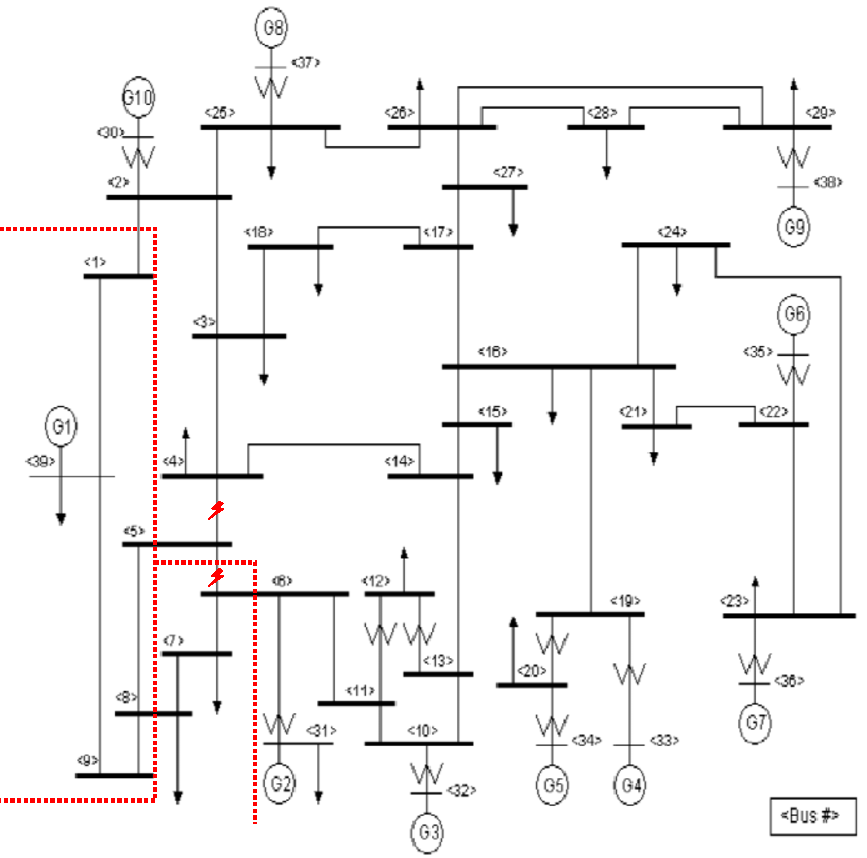
\includegraphics[width=0.475\linewidth]{Figs/IEEE39_slow_split.pdf}
        \label{subfig:split_slow}
    } \hfill
    \subfloat[System split following the (actual) fast sequence]{%
        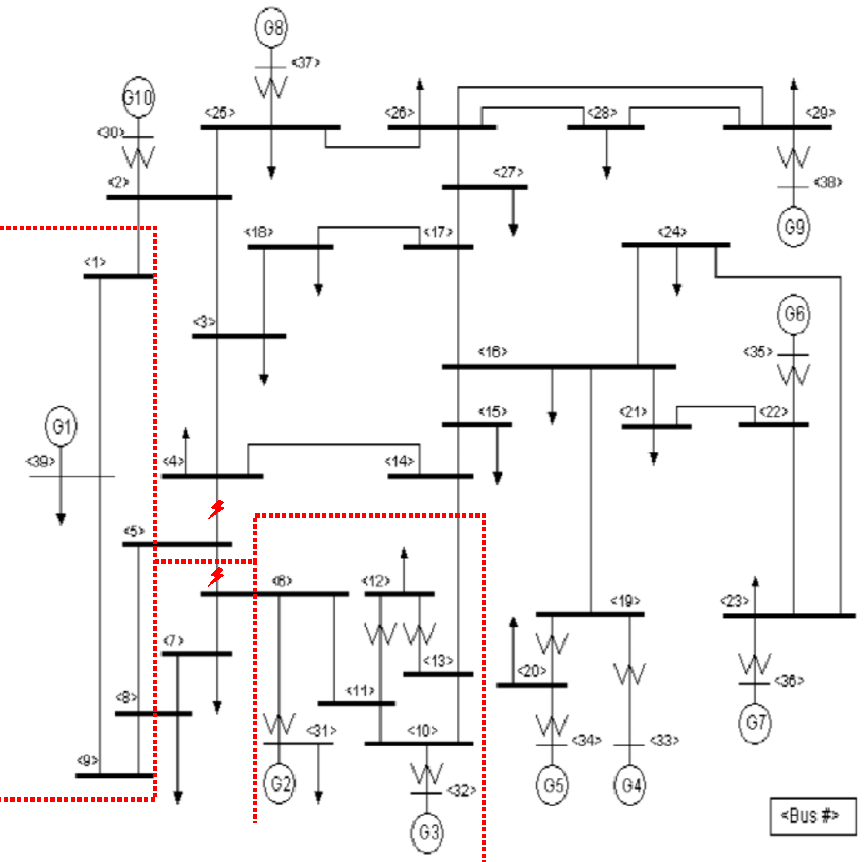
\includegraphics[width=0.475\linewidth]{Figs/IEEE39_fast_split.pdf}
        \label{subfig:split_fast}
    }
    \caption{Comparison of the consequences of the N-2 contingency of lines 5-6 and 6-7 in the slow and fast sequences (1-s restorative load case)}
    \label{fig:IEEE_split}
\end{figure}
}

% 6.15694 | 1-_2-1_AC_side2_DistanceSlow | Distance protection trip zone 2
% 6.22741 | 1-39-1_AC_side1_DistanceSlow | Distance protection trip zone 2
% 6.25709 | 5-_8-1_AC_side1_DistanceSlow | Distance protection trip zone 3
% 6.34501 | 8-_9-1_AC_side1_DistanceSlow | Distance protection trip zone 2
%
% 6.02905	13-14side1_Distance	Distance protection trip zone 3
% 6.05505 | 1-_2-1_AC_side2_DistanceFast | Distance protection trip zone 2
% 6.13181 | 5-_8-1_AC_side1_DistanceFast | Distance protection trip zone 3
% 6.134 | 1-39-1_AC_side1_DistanceFast | Distance protection trip zone 2
% 6.15187 | 4-14-1_AC_side2_DistanceFast | Distance protection trip zone 3
% 6.18391 | 8-_9-1_AC_side1_DistanceFast | Distance protection trip zone 2
%
% 6.02905	13-14side1_Distance	Distance protection trip zone 3
% 6.05505	1-2side2_Distance	Distance protection trip zone 2
% 6.13181	5-8side1_Distance	Distance protection trip zone 3
% 6.18407	8-9side1_Distance	Distance protection trip zone 2
% 8.27884	GEN___38_SM_Speed Under-speed protection trip
% 8.31923	GEN___37_SM_Speed	Under-speed protection trip
% 8.32712	GEN___30_SM_Speed	Under-speed protection trip
% 8.35866	GEN___33_SM_Speed	Under-speed protection trip
% 8.36521	GEN___35_SM_Speed	Under-speed protection trip
% 9.43916	23-24side1_Distance	Distance protection trip zone 2
% 9.55622	26-27side2_Distance	Distance protection trip zone 3
% 9.60304	16-17side1_Distance	Distance protection trip zone 3
% 9.81107	16-21side2_Distance	Distance protection trip zone 3
% 9.81712	GEN___33_SM_UVA	Under-voltage generator trip
% 9.84866	GEN___34_SM_UVA	Under-voltage generator trip

It can be noted that looking at the sequences of protection operations allows the indicator to perform significantly better than an indicator that would only consider the consequences of cascades. For example, Table~\ref{tab:indicator-consequence-based} shows the performance of an indicator that is true if the slower and faster sequences lead to different amount of load shedding%\footnote{Note that to estimate the load shedding, both sequences need to be simulated separately.}
. Such indicator indeed shows poor performance and misses between 20\% and 44\% (depending on the load model) of the sensitive contingencies.


\subsubsection{Causes of false negatives and false positives}
\label{sec:causesOfInaccuracy}

% 1s-restorative case, 3 FN
% _BUS___26-BUS___27-1_AC_end1-CB_end1-_BUS___26-BUS___29-1_AC
% Faster disconnection of GEN___38_SM_Speed that lost synchronism leads to less UFLS
% _BUS____2-BUS___25-1_AC_end2-CB_end2-_BUS___25-BUS___26-1_AC
% _BUS___26-BUS___29-1_AC_end2-CB_end1-_BUS___26-BUS___27-1_AC
% Same

% 5s, 1 FN
% _BUS___26-BUS___29-1_AC_end1-CB_end1-_BUS___26-BUS___27-1_AC
% Same

Table~\ref{tab:indicator} shows that the indicator misses 4 sensitive contingencies (3 false negatives in the 1s-restorative-load case, and 1 in the 5s-restorative one). In all those 4 cases, the difference between the slow and the (actual) fast sequences is that, in the fast sequence, generator 9 (bus 38) is disconnected faster by its protections after losing synchronism. This faster disconnection helps with frequency stability and leads to the activation of one less UFLS step. In the fast sequence estimated from the simulation of the slow one, this impact on the frequency behaviour is not caught, which leads to the false negatives. Using two simulations (one for the slower sequence and one for the faster sequence) would thus have lead to a null false negative rate (at the cost of an increase in computation time).

Table~\ref{tab:indicator} also shows that the indicator has a few false positives. It should however be noticed that false positives have a smaller impact that false negatives. Indeed, false negatives hide sensitive contingencies and lead to an inaccurate evaluation of their consequences (estimation from a single simulation while multiple MC simulations would be needed). However, false positives only cause unnecessary MC simulations which only affects computation time.

There are two causes for the occurrence of false positives. The first is that, in some cases, changing the order of protection operations does not impact the global evolution of the cascade. A typical example of this is when two distance protections operate to split the system in different points following an out-of-step condition. In this case, changing the order of protection operations will sometimes impact how the system splits and sometimes not.

The second cause is due to contingencies in which the operation of an additional protection system does not impact the consequences (in terms of load shedding). Most often, the protection system has no impact because it operates in an island that will collapse regardless of whether the protection system operates. % Both causes are each responsible for around 50\% of the false positives. % Also, one case where the ``new" protection that operates is Z3 instead of Z2 of the same protection -> actually not impact (most likely that Z2 will trip first anyway and that Z3 thus cannot trip after)


\section{Conclusion}
\label{sec:protection_conclusion}

Protection systems play a key role in maintaining highly-reliable power systems. However, they can sometimes misoperate, and they also impact (in positive and negative ways) the evolution of cascading outages. It is thus critical to model them adequately when performing probabilistic security assessments.

For this, it is important to first acknowledge the fact that protection systems can sometimes fail to clear faults in the normal way (i.e. by quickly disconnecting the faulted element), transforming mild N-1 contingencies into more severe N-k contingencies. This is because protection systems cannot be made 100\% dependable nor 100\% selective. Lack of dependability is mainly caused by the failure of individual protection elements (relays, breakers) and can be adequately modelled using standard reliability evaluation techniques such as fault trees and event trees. This is discussed in great detail in~\cite{GridPSA, Haarla}.

Lack of selectivity has more diverse causes, including design errors, incorrect settings, and as-left personnel errors~\cite{ProtectionMisoperationsBian2012} that are significantly harder to model. Most of the literature on the topic is rather old and is concerned with failure modes of legacy electromechanical relays that are no longer used. The update of failure models to digital relays is out of scope of this thesis but has recently been started in~\cite{Alexandre_PMAPS}. Statistics on the rate and causes of unselective protection behaviour at extra-high voltages (the ones most critical for security-related issues) would greatly help in evaluating the importance of unselective trips and to model them.

Beyond clearing the initial faults, protection systems also play a key role in how cascading outages propagate. As for fault clearing, lack of dependability or of selectivity can impact cascading outage evolution\footnote{Although, as will be shown in chapter~\ref{ch:DPSA}, the impact of lack of dependability after the initial fault clearing is relatively limited, except for SIPSs.}. However, even with perfectly reliable protection systems, it is difficult to predict how protection systems will impact the evolution of cascading outages. Indeed, during cascading outages, many protection systems might operate or be close to operate in a short window of time. Therefore, the propagation of cascading outages (and thus their final consequences) can be very sensitive to modelling uncertainties. In the literature, this has been studied using advanced MC techniques~\cite{SequencesRelaySobol, TwoLevelPSA}. However, MC simulations are computationally expensive which is problematic for the probabilistic security assessment of large systems that require to simulate many possible cascading outages. To alleviate this issue, this thesis proposes a simple indicator to predict which cascading outages are actually sensitive to protection-related uncertainties, so that MC simulations can be focused on these cases.

In conclusion, this chapter has discussed how to model N-k contingencies caused by protection misoperations and how to model the impact of protection systems on the evolution of cascading outages. The next step is thus to integrate this information into a comprehensive probabilistic security assessment framework. This is the objective of chapter~\ref{ch:DPSA}.
